\iffalse
\chapter{2009}
\author{AI24BTECH11022}
\section{ee}
\fi

\item An average-reading digital multimeter reads $10V$ when fed with a triangular wave, symmetric about the time-axis. For the same input an rms-reading meter will read\hfill(2009)
\begin{multicols}{2}
\begin{enumerate}
\item $\frac{20}{\sqrt{3}}$
\item $\frac{10}{\sqrt{3}}$
\item $20\sqrt{3}$
\item $10\sqrt{3}$
\end{enumerate}
\end{multicols}


\item Figure shows the extended view of a $2$ pole dc machine with $10$ armature conductors. Normal brush positions are shown by $A$ and $B$, placed at the interpolar axis. If the brushes are now shifted, in the direction of rotation, to $A^{\prime}$ and $B^{\prime}$ as shown, the voltage waveform $V_{A^{\prime}B^{\prime}}$ will resemble\hfill(2009)
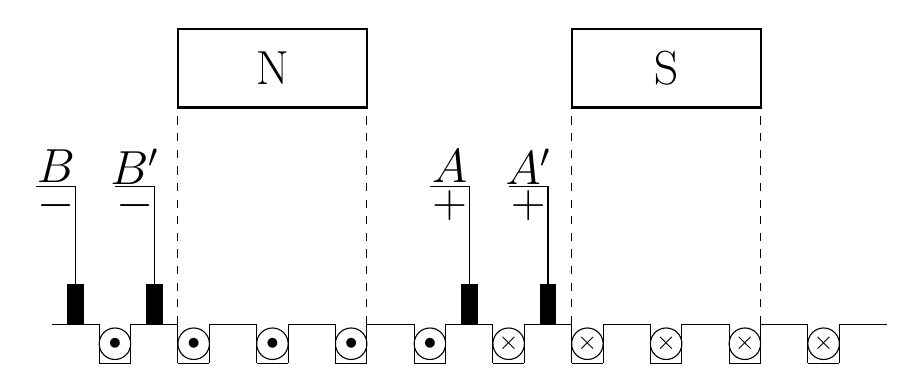
\begin{tikzpicture}
\draw[thick] (1.8,3) rectangle (4.2,4) node[midway] {N};
\draw[thick] (6.8,3) rectangle (9.2,4) node[midway] {S};
\draw[dashed] (1.8,0.25) -- (1.8,3);
\draw[dashed] (6.8,0.25) -- (6.8,3);
\draw[dashed] (4.2,0.25) -- (4.2,3);
\draw[dashed] (9.2,0.25) -- (9.2,3);
\foreach \x in {1,2,3,4,5,6,7,8,9,10} {\draw (\x,0) circle (0.2);}
\foreach \x in {1,2,3,4,5} {\draw (\x,0) node {\small $\bullet$};}
\foreach \x in {6,7,8,9,10} {\draw (\x,0) node {\small $\times$};}
\draw (0.2,0.25) -- (0.8,0.25);
\foreach \x in {1,2,3,4,5,6,7,8,9,10} {\draw (\x+0.2,0.25) -- (\x+0.8,0.25); \draw (\x-0.2,-0.25) -- (\x+0.2,-0.25);}
\foreach \x in {1,2,3,4,5,6,7,8,9,10} {\draw (\x-0.2,0.25) -- (\x-0.2,-0.25); \draw (\x+0.2,0.25) -- (\x+0.2,-0.25);}
\filldraw[black] (0.4,0.25) rectangle (0.6,0.75) node[midway,right] {};
\filldraw[black] (1.4,0.25) rectangle (1.6,0.75) node[midway,right] {};
\filldraw[black] (5.4,0.25) rectangle (5.6,0.75) node[midway,left] {};
\filldraw[black] (6.4,0.25) rectangle (6.6,0.75) node[midway,left] {};
\draw (0.5,0.75) -- (0.5,2) -- (0,2);
\draw (1.5,0.75) -- (1.5,2) -- (1,2);
\draw (5.5,0.75) -- (5.5,2) -- (5,2);
\draw (6.5,0.75) -- (6.5,2) -- (6,2);
\node at (0.25,2.25) {$B$};
\node at (1.25,2.25) {$B^{\prime}$};
\node at (5.25,2.25) {$A$};
\node at (6.25,2.25) {$A^{\prime}$};
\node at (0.25,1.75) {$-$};
\node at (1.25,1.75) {$-$};
\node at (5.25,1.75) {$+$};
\node at (6.25,1.75) {$+$};
\end{tikzpicture}

\begin{enumerate}
\item \begin{circuitikz}
\tikzstyle{every node}=[font=\LARGE]
\begin{scope}[rotate around={-14:(1.25,12.5)}]
\draw[domain=-0.75:1.25,samples=100,smooth] plot (\x,{1.6*sin(-1*\x r +1.25 r ) +12.5});
\end{scope}
\begin{scope}[rotate around={-14:(2.75,12.5)}]
\draw[domain=0.75:2.75,samples=100,smooth] plot (\x,{1.6*sin(-1*(\x-1.5) r +1.25 r ) +12.5});
\end{scope}
\begin{scope}[rotate around={-14:(4.25,12.5)}]
\draw[domain=2.25:4.25,samples=100,smooth] plot (\x,{1.6*sin(-1*(\x-3) r +1.25 r ) +12.5});
\end{scope}
\begin{scope}[rotate around={-14:(5.75,12.5)}]
\draw[domain=3.75:5.75,samples=100,smooth] plot (\x,{1.6*sin(-1*(\x-4.5) r +1.25 r ) +12.5});
\end{scope}
\begin{scope}[rotate around={-14:(7.25,12.5)}]
\draw[domain=5.25:7.25,samples=100,smooth] plot (\x,{1.6*sin(-1*(\x-6) r +1.25 r ) +12.5});
\end{scope}
\draw (1.25,12.5) -- (1.25,14.45);
\draw (2.75,12.5) -- (2.75,14.45);
\draw (4.25,12.5) -- (4.25,14.45);
\draw (5.75,12.5) -- (5.75,14.45);
\draw[->] (-0.4,12) -- (-0.4,15) node[above] {$V_{A'B'}$};
\draw[->] (-0.4,12) -- (8,12) node[right] {$\omega t$};
\draw[dashed] (1.25,12) -- (1.25,15);
\draw[dashed] (2.75,12) -- (2.75,15);
\draw[dashed] (4.25,12) -- (4.25,15);
\draw[dashed] (5.75,12) -- (5.75,15);
\draw[dashed] (7.25,12) -- (7.25,15);
\node at (1.25,11.5) {$0.2\pi$};
\node at (2.75,11.5) {$0.4\pi$};
\node at (4.25,11.5) {$0.6\pi$};
\node at (-0.5,11.5) {$0$};
\node at (5.75,11.5) {$0.8\pi$};
\node at (7.25,11.5) {$\pi$};
\end{circuitikz}


\item \begin{circuitikz}
\tikzstyle{every node}=[font=\LARGE]
\begin{scope}[rotate around={-14:(1.25,12.5)}]
\draw[domain=1.25:3.25,samples=100,smooth] plot (\x,{1.6*sin(1*\x r -1.25 r ) +12.5});
\end{scope}
\begin{scope}[rotate around={-14:(3.5,12.5)}]
\draw[domain=3.5:5.5,samples=100,smooth] plot (\x,{1.6*sin(1*(\x-2.25) r -1.25 r ) +12.5});
\end{scope}
\begin{scope}[rotate around={-14:(5.7
5,12.5)}]
\draw[domain=5.75:7.75,samples=100,smooth] plot (\x,{1.6*sin(1*(\x-4.5) r -1.25 r ) +12.5});
\end{scope}
\begin{scope}[rotate around={-14:(8,12.5)}]
\draw[domain=8:10,samples=100,smooth] plot (\x,{1.6*sin(1*(\x-6.75) r -1.25 r ) +12.5});
\end{scope}
\begin{scope}[rotate around={-14:(10.25,12.5)}]
\draw[domain=10.25:12.25,samples=100,smooth] plot (\x,{1.6*sin(1*(\x-9) r -1.25 r ) +12.5});
\end{scope}
\draw (3.5,12.5) -- (3.5,13.5);
\draw (5.75,12.5) -- (5.75,13.5);
\draw (8,12.5) -- (8,13.5);
\draw (10.25,12.5) -- (10.25,13.5);
\draw[->] (1.25,12) -- (12.75,12) node[above] {$\omega t$};
\draw[->] (1.25,12) -- (1.25,14) node[above] {$V_{A'B'}$};
\draw[dashed] (3.5,14) -- (3.5,12);
\draw[dashed] (5.75,14) -- (5.75,12);
\draw[dashed] (8,14) -- (8,12);
\draw[dashed] (10.25,14) -- (10.25,12);
\draw[dashed] (12.5,14) -- (12.5,12);
\node at (1.25,11.5) {$0$};
\node at (3.5,11.5) {$0.2\pi$};
\node at (5.75,11.5) {$0.4\pi$};
\node at (8,11.5) {$0.6\pi$};
\node at (10.25,11.5) {$0.8\pi$};
\node at (12.5,11.5) {$\pi$};
\end{circuitikz}

\item 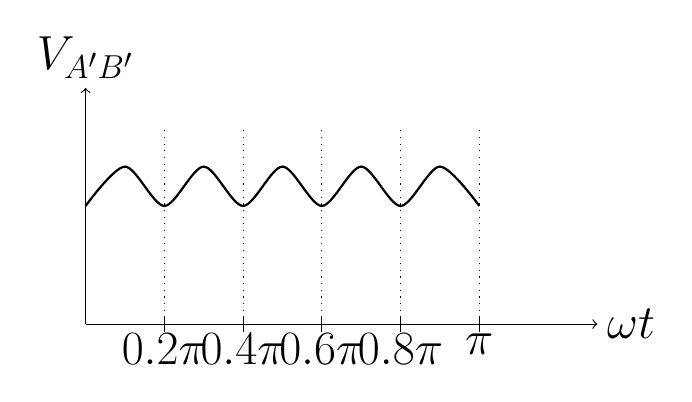
\begin{tikzpicture}
\draw[->] (0,0) -- (6.5,0) node[right] {$\omega t$};
\draw[->] (0,0) -- (0,3) node[above] {$V_{A'B'}$};
\foreach \x/\label in {1/0.2\pi,2/0.4\pi, 3/0.6\pi, 4/0.8\pi, 5/\pi}
{
\draw (\x,0.1) -- (\x,-0.1);
\node[below] at (\x,0) {$\label$};
}
    \draw[thick] plot[smooth] coordinates {
        (0,1.5)
        (0.5,2)
        (1,1.5)
        (1.5,2)
        (2,1.5)
        (2.5,2)
        (3,1.5)
        (3.5,2)
        (4,1.5)
        (4.5,2)
        (5,1.5)
    };
\foreach \x in {1,2,3,4,5}{
\draw[dotted] (\x,0) -- (\x,2.5);
}
\end{tikzpicture}

\item \begin{tikzpicture}
\draw (-0.5,13.5) -- (7.25,13.5);
\draw[->] (-0.4,12) -- (-0.4,15) node[above] {$V_{A'B'}$};
\draw[->] (-0.4,12) -- (8,12) node[right] {$\omega t$};
\draw[dashed] (1.25,12) -- (1.25,15);
\draw[dashed] (2.75,12) -- (2.75,15);
\draw[dashed] (4.25,12) -- (4.25,15);
\draw[dashed] (5.75,12) -- (5.75,15);
\draw[dashed] (7.25,12) -- (7.25,15);
\node at (1.25,11.5) {$0.2\pi$};
\node at (2.75,11.5) {$0.4\pi$};
\node at (4.25,11.5) {$0.6\pi$};
\node at (-0.5,11.5) {$0$};
\node at (5.75,11.5) {$0.8\pi$};
\node at (7.25,11.5) {$\pi$};
\end{tikzpicture}
\end{enumerate}
\vspace{10pt}

Common Data for Questions $51$ and $52$ :\\
\vspace{10pt}
\begin{circuitikz}
\draw (0,3) node[anchor=east] {} to[inductor] (2,3);
\draw (0,2) node[anchor=east] {} to[inductor] (2,2);
\draw (0,1) node[anchor=east] {} to[inductor] (2,1);
\draw (0,0) node[anchor=east] {} to[short] (1.25,0);
\draw (2,3) -- (2,0);
\node[anchor=east] at (1.75,-0.25) {S1};
\draw (3,3) to[inductor] (5,3) node[anchor=west] {};
\draw (3.5,2) to[inductor] (5,2) node[anchor=west] {};
\draw (3.5,1) to[inductor] (5,1) node[anchor=west] {};
\draw (5,3) -- (5,2.75);
\draw (5,2) -- (5,1.75);
\draw (3.5,2) -- (3.5,2.25);
\draw (3.5,1) -- (3.5,1.25);
\draw (3,3) -- (3,0);
\draw (3.75,0) -- (5,0);
\draw (5,2.75) -- (3.5,2.25);
\draw (5,1.75) -- (3.5,1.25);
\draw (5,1) -- (5,0);
\node[anchor=west] at (3.25,-0.25) {S2};
\draw (0,3) -- ++(-0.5,0) node[circle, draw, fill=black, inner sep=1pt] {};
\draw (0,2) -- ++(-0.5,0) node[circle, draw, fill=black, inner sep=1pt] {};
\draw (0,1) -- ++(-0.5,0) node[circle, draw, fill=black, inner sep=1pt] {};
\draw (0,0) -- ++(-0.5,0) node[circle, draw, fill=black, inner sep=1pt] {};
\draw (5,3) -- ++(0.5,0) node[circle, draw, fill=black, inner sep=1pt] {};
\draw (5,2) -- ++(0.5,0) node[circle, draw, fill=black, inner sep=1pt] {};
\draw (5,1) -- ++(0.5,0) node[circle, draw, fill=black, inner sep=1pt] {};
\node at (-0.75,0) {N};
\node at (-0.75,1) {C};
\node at (-0.75,2) {B};
\node at (-0.75,3) {A};
\node at (5.75,1) {c};
\node at (5.75,2) {b};
\node at (5.75,3) {a};
\draw (1.25,0.25) -- (1.75,0);
\draw (1.75,0) -- (2,0);
\draw (3.75,0.25) -- (3.25,0);
\draw (3.25,0) -- (3,0);
\end{circuitikz}


The star-delta transformer shown above is excited on the star side with a balanced, $4-wire$, $3-phase$, sinusoidal voltage supply of rated magnitude. The transformer is under no load condition.\\

\item With both $S1$ and $S2$ open, the core flux waveform will be\hfill(2009)
\begin{multicols}{2}
\begin{enumerate}
\item a sinusoid at fundamental frequency
\item flat-topped with third harmonic
\item peaky with third-harmonic
\item none of these
\end{enumerate}
\end{multicols}


\item With $S2$ closed and $S1$ open, the current waveform in the delta winding will be\hfill(2009)
\begin{multicols}{2}
\begin{enumerate}
\item a sinusoid at fundamental frequency
\item flat-topped with third harmonic
\item only third-harmonic
\item none of these
\end{enumerate}
\end{multicols}


Common Data for Questions $53$ and $54$ :\\

The circuit diagram shows a two-winding, lossless transformer with no leakage flux, excited from a current source, $i\brak{t}$, whose waveform is also shown. The transformer has a magnetizing inductance of $\frac{400}{\pi}mH$.
\begin{circuitikz}
\draw (0,0) to[isource, l=$i(t)$] (0, 2);
\draw (2,2) to[cute inductor] (2,0);
\draw (0,0) to (2,0);
\draw (0,2) to (2,2);
\draw[ultra thick] (2.3,0.5) -- (2.3,1.5);
\draw[ultra thick] (2.6,0.5) -- (2.6,1.5);
\draw (3,0) to[cute inductor] (3,2) to (5,2) to (5,1.75);
\draw (5,1.5) to[R=$30\Omega$] (5,0) to (3,0);
\draw (5,1.75) to (5.25,1.5);
\node at (2.5,2.5) {1:1};
\draw (0,0) node[circle, draw, fill=white, inner sep=1pt] {};
\draw (0,2) node[circle, draw, fill=white, inner sep=1pt] {};
\draw (4,0) node[circle, draw, fill=black, inner sep=1pt] {};
\draw (4,2) node[circle, draw, fill=black, inner sep=1pt] {};
\node at (4,2.25) {A};
\node at (4,-0.25) {B};
\node at (5.5,1.5) {S};
\end{circuitikz}

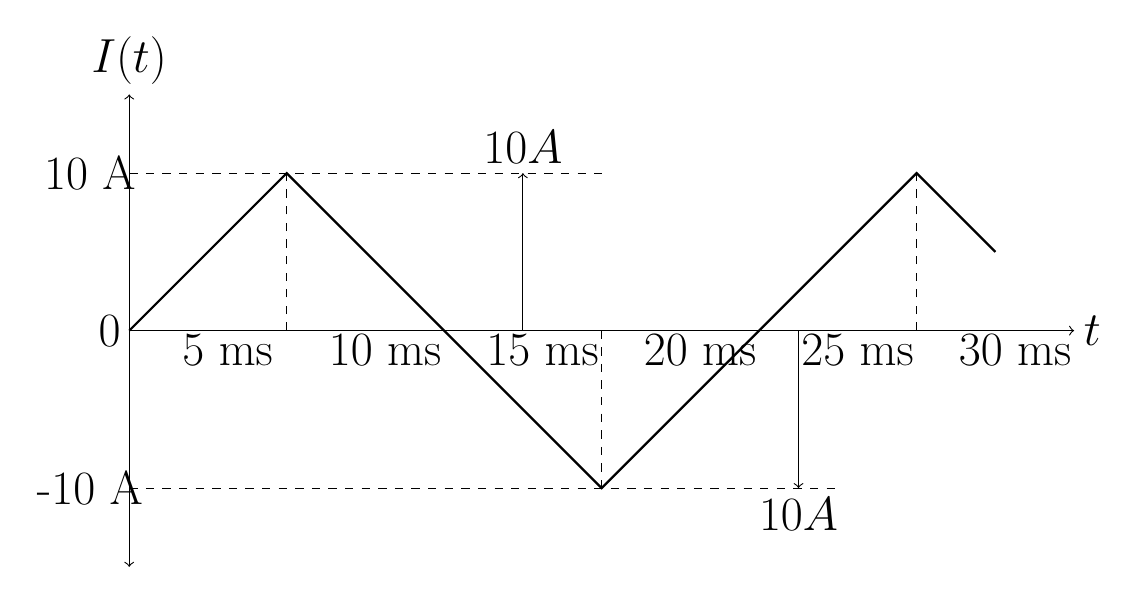
\begin{tikzpicture}
\draw[->] (0,0) -- (12,0) node[right] {$t$};
\draw[->] (0,0) -- (0,3) node[above] {$I(t)$};
\draw[->] (0,0) -- (0,-3);
\node at (-0.5,2) {10 A};
\node at (-0.5,-2) {-10 A};
\node at (1.25,-0.25) {5 ms};
\node at (3.25,-0.25) {10 ms};
\node at (5.25,-0.25) {15 ms};
\node at (7.25,-0.25) {20 ms};
\node at (9.25,-0.25) {25 ms};
\node at (11.25,-0.25) {30 ms};
\node at (-0.25,0) {0};
\draw[dashed] (2,0) -- (2,2);
\draw[dashed] (6,0) -- (6,-2);
\draw[dashed] (10,0) -- (10,2);
\draw[dashed] (0,2) -- (6,2);
\draw[dashed] (0,-2) -- (9,-2);
\draw[thick] (0,0) -- (2,2) -- (6,-2)  -- (10,2) -- (11,1);
\draw[->] (5,0) -- (5,2) node[above] {$10A$};
\draw[->] (8.5,0) -- (8.5,-2) node[below] {$10A$};
    
\end{tikzpicture}

\item The peak voltage across A and B, with S open is\hfill(2009)
\begin{multicols}{2}
\begin{enumerate}
\item $\frac{400}{\pi}V$
\item $800V$
\item $\frac{4000}{\pi}V$
\item $\frac{800}{\pi}V$
\end{enumerate}
\end{multicols}


\item If the waveform of $i\brak{t}$ is changed to $i\brak{t}=10\sin{100\pi t}A$, the peak voltage across $A$ and $B$ with $S$ closed is\hfill(2009)
\begin{multicols}{2}
\begin{enumerate}
\item $400V$
\item $240V$
\item $320V$
\item $160V$
\end{enumerate}
\end{multicols}


Common Data for Questions $55$ and $56$:\\

A system is described by the following state and output equations
$$\frac{dx_{1}\brak{t}}{dt}=-3x_{1}\brak{t}+x_{2}\brak{t}+2u\brak{t}$$
$$\frac{dx_{2}\brak{t}}{dt}=-2x_{2}\brak{t}+u\brak{t}$$
$$y\brak{t}=x_{1}\brak{t}$$
where $u\brak{t}$ is the input and $y\brak{t}$ is the output\\

\item The system transfer function is\hfill(2009)
\begin{multicols}{2}
\begin{enumerate}
\item $\frac{s+2}{s^{2}+5s-6}$
\item $\frac{s+3}{s^{2}+5s+6}$
\item $\frac{2s+5}{s^{2}+5s+6}$
\item $\frac{2s-5}{s^{2}+5s-6}$
\end{enumerate}
\end{multicols}


\item The state-transition matrix of the above system is\hfill(2009)
\begin{multicols}{2}
\begin{enumerate}
\item $\begin{bmatrix} e^{-3t}&0\\e^{-2t}+e^{-3t}&e^{-2t} \end{bmatrix}$
\item $\begin{bmatrix} e^{-3t}&e^{-2t}-e^{-3t}\\0&e^{-2t} \end{bmatrix}$
\item $\begin{bmatrix} e^{-3t}&e^{-2t}+e^{-3t}\\0&e^{-2t} \end{bmatrix}$
\item $\begin{bmatrix} e^{3t}&e^{-2t}-e^{-3t}\\0&e^{-2t} \end{bmatrix}$
\end{enumerate}
\end{multicols}


Statement for Linked Answer Questions $57$ and $58$ :\\
\begin{circuitikz}
\draw[thick] (3.8,0) -- (3.8,3);
\draw[thick] (4.2,0) -- (4.2,3);
\draw (2,3) node[anchor=east] {A} to[short] (3,3) to[cute inductor] (3,0);
\draw (2,0) node[anchor=east] {B} to[short] (3,0);
\draw (5,3) to[cute inductor] (5,0) to[short] (6,0) node[anchor=west] {D};
\draw (5,3) to[short] (6,3) node[anchor=west] {C};
\node[anchor=west] at (1.75,1.5) {Coil 1};
\node[anchor=west] at (5.25,1.5) {Coil 2};
\draw (2,3) node[circle, draw, fill=black, inner sep=1pt] {};
\draw (2,0) node[circle, draw, fill=black, inner sep=1pt] {};
\draw (6,3) node[circle, draw, fill=black, inner sep=1pt] {};
\draw (6,0) node[circle, draw, fill=black, inner sep=1pt] {};
\end{circuitikz}

The figure above shows coils $1$ and $2$, with dot markings as shown, having $4000$ and $6000$ turns respectively. Both the coils have a rated current of $25A$. Coil $1$ is excited with single phase, $400V$, $50Hz$ supply.\\

\item The coils are to be connected to obtain a single phase, $400/1000V$, auto-transformer to drive a load of $10kVA$. Which of the options given should be exercised to realize the required auto-transformer?\hfill(2009)
\begin{multicols}{2}
\begin{enumerate}
\item Connect $A$ and $D$; Common $B$
\item Connect $B$ and $D$; Common $C$
\item Connect $A$ and $C$; Common $B$
\item Connect $A$ and $C$; Common $D$
\end{enumerate}
\end{multicols}

\item In the autotransformer obtained in Question $57$, the current in each coil is\hfill(2009)
\begin{multicols}{2}
\begin{enumerate}
\item Coil-$1$ is $25A$ and Coil-$2$ is $10A$
\item Coil-$1$ is $10A$ and Coil-$2$ is $25A$
\item Coil-$1$ is $10A$ and Coil-$2$ is $15A$
\item Coil-$1$ is $15A$ and Coil-$2$ is $10A$
\end{enumerate}
\end{multicols}


Statement for Linked Answer Questions $59$ and $60$ :\\
\begin{circuitikz}[american voltages]
\draw (0,0) to[vsource, v=$5V$, invert] (0,3)to[R=2k$\Omega$] (3,3);
\draw (3,3) to[R=2k$\Omega$] (3,0);
\draw (3,3) to[controlled voltage source, l_=3V$_{AB}$] (6,3)to[R=1k$\Omega$] (6,0);
\node at (7,3) {A};
\node at (7,0) {B};
\draw (6,3) -- ++(0.5,0);
\draw (6,0) -- ++(0.5,0);
\draw (6,3) -- ++(0.5,0) node[circle, draw, fill=white, inner sep=1pt] {};
\draw (6,0) -- ++(0.5,0) node[circle, draw, fill=white, inner sep=1pt] {};
\draw (0,0) -- (6,0);
\end{circuitikz}

\item For the circuit given above, the Thevenin's resistance across the terminals $A$ and $B$ is\hfill(2009)
\begin{multicols}{2}
\begin{enumerate}
\item $0.5k\ohm$
\item $0.2k\ohm$
\item $1k\ohm$
\item $0.11k\ohm$
\end{enumerate}
\end{multicols}


\item For the circuit given above, the Thevenin's voltage across the terminals $A$ and $B$ is\hfill(2009)
\begin{multicols}{2}
\begin{enumerate}
\item 1.25 V
\item 0.25 V
\item 1 V
\item 0.5 V
\end{enumerate}
\end{multicols}